% !TEX program = xelatex
\documentclass[12pt]{ctexart}
\usepackage{amsfonts,amssymb}
\usepackage{booktabs}
\usepackage{graphicx}
\usepackage{amsmath}
\usepackage{listings}
\usepackage{geometry}
\usepackage[usenames,dvipsnames]{xcolor}
\usepackage{setspace}
\usepackage{hyperref}
\usepackage{float}
\setstretch{1.1} 
\geometry{a4paper}
\geometry{top=2cm} 
\geometry{bottom=1cm} 
\geometry{left=1.5cm, right=1.5cm}
\tolerance=1000
\definecolor{mygreen}{rgb}{0,0.6,0}
\definecolor{mygray}{rgb}{0.5,0.5,0.5}
\definecolor{mymauve}{rgb}{0.58,0,0.82}
\lstset{ %
backgroundcolor=\color{white},   % choose the background color
basicstyle=\footnotesize\ttfamily,        % size of fonts used for the code
columns=fullflexible,
keepspaces=true,
inputencoding=utf8,
extendedchars=true, 
breaklines=true,                 % automatic line breaking only at whitespace
captionpos=b,                    % sets the caption-position to bottom
tabsize=4,
commentstyle=\color{mygreen},    % comment style
escapeinside={\%*}{*)},          % if you want to add LaTeX within your code
keywordstyle=\color{blue},       % keyword style
stringstyle=\color{mymauve}\ttfamily,     % string literal style
frame=single,
rulesepcolor=\color{red!20!green!20!blue!20},
% identifierstyle=\color{red},
language=c++,
}
\newcommand*{\dif}{\mathop{}\!\mathrm{d}}
\author{SSerxhs}
\title{SSerxhs 的 ICPC 模板}

\begin{document}

\maketitle

\centerline{ver: 3.12.2}

\tableofcontents

\newpage

\section{前言}

此模板的初衷是个人使用，因此已有的模板可能未列出。建议结合 Heltion 模板和 HDU 模板使用。

模板需要的版本为 cpp17 或 cpp20。

大部分情况下，涉及取模的都需要使用 \verb|unsigned long long|，即使类型名是 \verb|ll|。这是因为值域较大有利于合理减少取模次数。目前，大部分都已经修改为 \verb|ull|。

\verb|optional| 的用法：一个 \verb|optional| 变量 \verb|r| 可以用 \verb|if (r)| 判断其是否有值。取出值的方法是 \verb|*r|。常见于包含无解又包含空集解的代码中，便于区分无解和空集解。

\verb|rev| 宏通常用于数据结构中，正向信息是否与反向信息相同，若定义了宏则表示不同。例如矩阵乘法需要定义，而区间求和则不需要。定义后额外统计信息，会慢一点点。

常见的被漏掉的初始代码：
\lstinputlisting{code/前言/前言.cpp}

常见的缺漏算法：

回文自动机，最小树形图。

\newpage

\section{数据结构}

\subsection{树状数组}

支持单点修改、求前缀和、二分前缀和大于等于 $x$ 的第一个位置。

\lstinputlisting{code/数据结构/树状数组.cpp}

\subsection{线段树}

包含标记的线段树，支持线段树上二分，采用左闭右闭。但只支持求左侧第一个符合条件的下标。

要求：具有 \verb|info+info|，\verb|info+=tag|，\verb|tag+=tag|。\verb|info|，\verb|tag| 需要有默认构造，但不必有正确的值。

示例的 \verb|tag| 和 \verb|info| 是区间加区间覆盖区间历史最大值。

对于线段树上二分，如果你要 \verb|check| 的是前缀，可以在 \verb|false| 时加入信息。

例如查找前缀和大于等于 $s$ 的第一个下标，可以写成

\lstinputlisting{code/数据结构/线段树.cpp}

\lstinputlisting{code/数据结构/线段树_2.cpp}


\subsection{珂朵莉树}
支持区间赋值、单点访问。维护每个连续段的范围和值。

如果希望维护所有连续段的整体信息（如长度的最大值），修改 \verb|add| 和 \verb|del| 函数即可，分别表示连续段被加入和被删去。

特别注意一开始 \verb|insert| 的不会触发 \verb|add|，只有 \verb|modify| 会触发。
\lstinputlisting{code/数据结构/珂朵莉树.cpp}


\subsection{带删堆}

本质是额外维护一个堆 \verb|q| 表示要被删除的元素，当 \verb|p| 的最值和 \verb|q| 一样时删除。

需要保证每次 \verb|pop| 的元素都存在于堆中。

本代码的用法和 \verb|priority_queue| 一致。

\lstinputlisting{code/数据结构/带删堆.cpp}
\subsection{前 $k$ 大的和}

本质是用小根堆维护前 $k$ 大的数，用大根堆维护其余数。

如果需要支持删除，结合前面一个使用，或者直接用 \verb|multiset| 进行 \verb|extract|。

为了方便起见，直接给出支持删除的版本，并且使用 \verb|long long|。如果不需要支持删除，类型改为优先队列并去掉 \verb|pop| 函数即可。

注意：复杂度为 $O(|k-k'|)$，其中 $k'$ 是上一次询问的 $k$。也就是说，多组询问时询问的 $k$ 的差值应该尽可能小。

其用法与 \verb|priority_queue| 保持一致，可以用同样的方法改写成前 $k$ 小。

\lstinputlisting{code/数据结构/前 k 大的和.cpp}

\subsection{左偏树/可并堆}

建议不要使用。\verb|pb_ds| 可以替代这个功能。我完全没有使用过这个板子。

$O((n+q)\log n)$，$O(n)$。

\lstinputlisting{code/数据结构/左偏树_可并堆.cpp}

\subsection{树状数组区间加区间求和}

本质：$a_n$ 区间加等价于差分数组 $d_n$ 的单点加。

$\sum\limits_{i=1}^ma_i =\sum\limits_{i=1}^m\sum\limits_{j=1}^id_j=\sum\limits_{j=1}^md_j(m-j+1)=((m+1)\sum\limits_{j=1}^md_j)-(\sum\limits_{j=1}^mjd_j)$。

分别维护 $d_j$ 和 $jd_j$ 的前缀和。

$O(n)\sim O(q\log n)$，$O(n)$。

\lstinputlisting{code/数据结构/树状数组区间加区间求和.cpp}

\subsection{二维树状数组矩形加矩形求和}

本质还是差分，只不过这次要维护 $d_{i,j},d_{i,j}i,d_{i,j}j,d_{i,j}ij$。

$O(n^2+q\log^2n)$，$O(n^2)$

\lstinputlisting{code/数据结构/二维树状数组矩形加矩形求和.cpp}

\subsection{带修莫队}

按照 $n^{\frac{2}{3}}$ 分块，排序关键字是 $l,r,t$ 所在的块（$t$ 是版本号，每次修改都会增加一个版本），可以奇偶分块优化。

相比于传统莫队多了一个 \verb|modify|。这里只给出参考代码，功能是带修区间数颜色。

$O(n^{\frac {5}{3}})$，$O(n)$。

\lstinputlisting{code/数据结构/带修莫队.cpp}

\subsection{二次离线莫队}

直接摘录题解，用途不大。

$O(n\sqrt n)$，$O(n)$。

珂朵莉给了你一个序列 $a$，每次查询给一个区间 $[l,r]$，查询 $l \leq i< j \leq r$，且 $a_i \oplus a_j$ 的二进制表示下有 $k$ 个 $1$ 的二元组 $(i,j)$ 的个数。$\oplus$ 是指按位异或。

二次离线莫队，通过扫描线，再次将更新答案的过程离线处理，降低时间复杂度。假设更新答案的复杂度为 $O(k)$，它将莫队的复杂度从 $O(nk\sqrt n)$ 降到了 $O(nk + n\sqrt n)$，大大简化了计算。
设 $x$ 对区间 $[l,r]$ 的贡献为 $f(x,[l,r])$，我们考虑区间端点变化对答案的影响：以 $[l..r]$ 变成 $[l..(r+k)]$ 为例，$\forall x \in [r+1,r+k]$ 求 $f(x,[l,x-1])$。
我们可以进行差分：$f(x,[l,x-1])=f(x,[1,x-1])-f(x,[1,l-1])$，这样转化为了一个数对一个前缀的贡献。保存下来所有这样的询问，从左到右扫描数组计算就可以了。
但是这样做，空间是 $O(n\sqrt n)$ 的，不太优秀，而且时间常数巨大。。
这样的贡献分为两类：

1. 减号左边的贡献永远是一个前缀 和它后面一个数的贡献。这可以预处理出来。
2. 减号右边的贡献对于一次移动中所有的 $x$ 来说，都是不变的。我们打标记的时候，可以只标记左右端点。

这样，减小时间常数的同时，空间降为了 $O(n)$ 级别。是一个很优秀的算法了。处理前缀询问的时候，我们利用异或运算的交换律，即 $a~\mathrm{xor}~b=c \Longleftrightarrow a~\mathrm{xor}~c=b$
开一个桶 $t$，$t[i]$ 表示当前前缀中与 $i$ 异或有 $k$ 个数位为 $1$ 的数有多少个。
则每加入一个数 $a[i]$，对于所有 $\mathrm{popcount}(x)=k$ 的 $x$，$t[a[i]\operatorname{xor}x]\gets t[a[i]\operatorname{xor}x]+1$ 即可。

\lstinputlisting{code/数据结构/二次离线莫队.cpp}

\subsection{回滚莫队}

不删除的莫队，比如求 $\max$。

做法：块内询问暴力。对于 $l$ 所在块相同的询问，按照 $r$ 升序排序，并且将左指针固定在 $l$ 所在块的最右侧。（由于块内询问暴力，这不会导致左指针更大）

回答每个询问的时候，先右端点右移到 $r$，然后左端点左移到 $l$。询问完成后，把左端点移回去。移回去的过程虽然涉及删除，但不需要维护答案变成什么了（因为在左端点左移之前已经求过了）。换句话说，相当于“撤销”而不是删除，完全可以记录移动过程中的所有变化来撤销。

$O(n\sqrt n)$，$O(n)$。

\lstinputlisting{code/数据结构/回滚莫队.cpp}

\subsection{李超树}

题意：插入线段，查询某个 $x$ 的最大 $y$（输出最小编号）

算法核心：修改时，线段树每个点只维护在中点取值最大的线段，中点取值较小的线段只会在至多一侧有用，递归下去插入，复杂度 $O(\log^2)$。查询时询问线段树上 $\log$ 个点的线段中最大的。

\lstinputlisting{code/数据结构/李超树.cpp}

\subsection{李超树（动态开点）}
\lstinputlisting{code/数据结构/李超树(动态开点).cpp}


\subsection{线性基}

$O((n+q)\log a)$，$O(n\log a)$。

\lstinputlisting{code/数据结构/线性基.cpp}

\subsection{splay}

指针版。

$O(n)$，$O((n+q)\log n)$。

\lstinputlisting{code/数据结构/splay.cpp}

\subsection{fhq-treap}

洛谷模板：普通平衡树。

$O((n+q)\log n)$，$O(n)$。

\lstinputlisting{code/数据结构/fhq-treap.cpp}

\subsection{笛卡尔树的线性建树}

$p[1,2,\ldots,n]$ 是原序列，\verb|c| 表示子结点。

笛卡尔树满足堆性质（权值小于等于子结点权值），并且中序遍历是原序列。

$O(n)$，$O(n)$。

\lstinputlisting{code/数据结构/笛卡尔树的线性建树.cpp}

\subsection{扫描线}

求矩形并的面积和周长（包括内周长）

$O((n+q)\log n)$，$O(n+q)$。

\lstinputlisting{code/数据结构/扫描线.cpp}

\subsection{Segmenttree Beats!}
核心是 P（tag） 和 Q（info） 的维护。线段树部分是套的模板，并非全都有用。
\begin{enumerate}
	\item $l,r,k$：对于所有的 $i\in[l,r]$，将 $A_i$ 加上 $k$（$k$ 可以为负数）。
	\item $l,r,v$：对于所有的 $i\in[l,r]$，将 $A_i$ 变成 $\min(A_i,v)$。
	\item $l,r$：求 $\sum\limits_{i=l}^{r}A_i$。
	\item $l,r$：对于所有的 $i\in[l,r]$，求 $A_i$ 的最大值。
	\item $l,r$：对于所有的 $i\in[l,r]$，求 $B_i$ 的最大值。
\end{enumerate}
其中 $B_i$ 是 $A_i$ 的历史最大值。
\lstinputlisting{code/数据结构/Segmenttree Beats!.cpp}

\subsection{$k$-d 树（二进制分组）}

均摊 $O(\log ^2n)$ 插入，$O(\sqrt n)$ 矩形查询。

\lstinputlisting{code/数据结构/k-d 树(二进制分组).cpp}

\subsection{双端队列全局查询}

对一个支持结合律的信息 T，维护 \verb|deque| 内信息的和。总复杂度线性。

\lstinputlisting{code/数据结构/双端队列全局查询.cpp}

\subsection{静态矩形加矩形和}

\lstinputlisting{code/数据结构/静态矩形加矩形和.cpp}

\subsection{线段树分裂}

\lstinputlisting{code/数据结构/线段树分裂.cpp}

\subsection{手写 bitset}

\lstinputlisting{code/数据结构/手写 bitset.cpp}

\subsection{区间众数}

\lstinputlisting{code/数据结构/区间众数.cpp}

\subsection{表达式树}

传入表达式，输出表达式树。

输入的第二个参数是全体括号以外的运算符，每个运算符要记录字符优先级和是否右结合。优先级数字越大，越优先计算，且优先级必须为正整数。

输出的第一个参数是子结点数组，第二个参数是每个结点对应的字符，第三个参数是根。结点编号从 $1$ 开始。

输出的表达式树满足每个结点对应一个字符。若包含数字串，则视为相邻数码之间加一个井号，表示“数码链接”这个运算符。你不需要，也不应该手动加入这个井号。

如果表达式非法，将返回根为 $0$。不允许一元运算符（负号），不允许省略乘号，不允许出现字母（除非字母是运算符）。

如果需要支持字母作为数字，修改所有包含 \verb|isdigit| 的部分。

由于存在“数码链接”，在 \verb|dfs| 树的时候最好记录一下子树大小，便于链接时计算（你不能在链接时直接看右子树的数字大小，因为有可能有前导 $0$）。

\lstinputlisting{code/数据结构/表达式树.cpp}

\subsection{区间排序区间复合}

时空 $O((n+m)\log V)$，其中 $V$ 是排序关键字的值域，要求排序关键字唯一。实际效率较低，$10^5$ 要 1.2s。

构造函数传入排序关键字与信息，以及排序关键字的值域范围。

与其他板子不同的是，所有区间都是左闭右开的，下标从 $0$ 开始。

\lstinputlisting{code/数据结构/区间排序区间复合.cpp}
\newpage

\section{数学}


\subsection{矩阵类（较新）}

\lstinputlisting{code/数学/矩阵类(较新).cpp}


\subsection{在线 $O(1)$ 逆元}

预处理复杂度为 $O(p^{\frac{2}{3}})$。

\lstinputlisting{code/数学/在线 O(1) 逆元.cpp}

\subsection{Strassen 矩阵乘法}

没用，不如卡常。$O(n^{\log_27})$。

\lstinputlisting{code/数学/Strassen 矩阵乘法.cpp}

\subsection{扩展欧拉定理}

求 $a\uparrow\uparrow b \bmod c$。前面的 Prime 命名空间只是求 $\varphi$ 用的。

特别注意，这里的 \verb|i64| 不是无符号。

\lstinputlisting{code/数学/扩展欧拉定理.cpp}

\subsection{exgcd}

$O(\log p)$，$O(\log p)$。

递归版：

\lstinputlisting{code/数学/exgcd.cpp}

递推版：

\lstinputlisting{code/数学/exgcd_2.cpp}

\subsection{exCRT}

CRT：设 $M=\prod\limits_{i=1}^nm_i$，$t_i\times \dfrac {M}{m_i}\equiv 1\pmod {m_i}$，则 $x\equiv \sum\limits_{i=1}^na_it_i\dfrac {M}{m_i}$。

以下为 exCRT，与 CRT 无关。实现了一个类 \verb|Q|，表示一条方程，支持合并。

\lstinputlisting{code/数学/exCRT.cpp}


\subsection{exBSGS}

$O(\sqrt n)$。哈希表 \verb|ht| 可以用 \verb|map| 代替。

\lstinputlisting{code/数学/exBSGS.cpp}

\subsection{exLucas}

求组合数。

\lstinputlisting{code/数学/exLucas.cpp}

\subsection{杜教筛}

求 $\varphi(n)$ 的前缀和。

核心：构造 $g$ 满足 $h(n)=\sum\limits_{d|n}f(d)g(\frac{n}{d})$ 容易计算，

则有 $\sum\limits_{i=1}^n h(i)=\sum\limits_{i=1}^n g(i)\sum\limits_{j=1}^{\lfloor n/i\rfloor}f(j)$，

故 $g(1)\sum\limits_{j=1}^n f(j)=\sum\limits_{i=1}^n h(i)-\sum\limits_{i=2}^n g(i)\sum\limits_{j=1}^{\lfloor n/i\rfloor}f(j)$，

则 $f$ 前缀和可以递归求解。

\lstinputlisting{code/数学/杜教筛.cpp}

\subsection{$\mu^2(n)$ 前缀和}

$10^{18}$，0.46s。

$\mu^2(n)=\sum\limits_{d^2|n}\mu(d)$

\lstinputlisting{code/数学/mu^2(n) 前缀和.cpp}
\subsection{线性规划}
用法：构造函数指明目标函数系数，\verb|add| 函数增加限制。额外的限制是 $x_i\ge 0$。
\lstinputlisting{code/数学/线性规划.cpp}

\subsection{线性插值（$k$ 次幂和）}

$O(m)$，$O(m)$。


\lstinputlisting{code/数学/线性插值(k 次幂和).cpp}
\subsection{幂乘等比}

$\sum\limits_{i=0}^{n-1}x^ii^d$ 以及 $\sum\limits_{i=0}^{\infty}x^ii^d$

$O(d)$。

\lstinputlisting{code/数学/幂乘等比.cpp}


\subsection{原根}

你应该传入的是模数 $m$ 和你提供的 \verb|getw| 函数，用于分解质因数。

以下以我的 pollard rho 模板为例。如果在现场赛且范围不大，手动求出更为方便。

定理：只有 $2,4,p^k,2p^k$ 有原根。因此可以优化到只分解一次，但没必要。

\lstinputlisting{code/数学/原根.cpp}

\subsection{筛全部原根}

\lstinputlisting{code/数学/筛全部原根.cpp}

\subsection{高斯消元（浮点数）}

$O(n^3)$，$O(n^2)$。

\lstinputlisting{code/数学/高斯消元(浮点数).cpp}

\subsection{行列式求值（任意模数）}

$O(n^3)$，$O(n^2)$。

原理：辗转相除。注意这个 $\log p$ 并不在 $n^3$ 上。

\lstinputlisting{code/数学/行列式求值(任意模数).cpp}

\subsection{BM/稀疏矩阵系列}

BM：给定 $\{a\}$，求最短的 $\{r\}$ 满足 $\sum\limits_{j=0}^{m-1} a_{i-j-1}r_j=a_i$。

\verb|safe| 宏用于验证结果正确性，可不定义。实现了稀疏矩阵的行列式和求解方程组。

\lstinputlisting{code/数学/BM_稀疏矩阵系列.cpp}



\subsection{Min\_25筛}

$f(p^k)=p^k(p^k-1)$，求 $\sum\limits_{i=1}^n f(i)$。这个的原理我了解的不多，因此没有更多注释。

\lstinputlisting{code/数学/Min__25筛.cpp}

这是一个常数较小的版本，实现的是质数个数。需要注意评测机 \verb|double| 性能。

\lstinputlisting{code/数学/Min__25筛_2.cpp}

\subsection{光速乘}

$O(n2^n)$，$O(2^n)$。


\lstinputlisting{code/数学/光速乘.cpp}

\subsection{二次剩余}

\lstinputlisting{code/数学/二次剩余.cpp}

\subsection{$k$ 次剩余}
\lstinputlisting{code/数学/k 次剩余.cpp}

网上的超快版本

\lstinputlisting{code/数学/k 次剩余_2.cpp}

\subsection{FWT/子集卷积}

$O(n2^n)$，$O(2^n)$。注意全都是无符号的。

\lstinputlisting{code/数学/FWT_子集卷积.cpp}

\subsection{NTT}

一种较快的 NTT（尤其是对于卷积以外的用途），但不推荐在不熟悉的情况下直接使用。一般的卷积可以参照字符串部分通配符的字符串匹配，其余的用途可以参照其他板子。

如果确实需要卡常，建议先抄写需要的函数，并递归地找到需要补的内容。

注意事项：所有 \verb|ull| 为无符号。始终保证数组大小为 $2^n$，不应当使用 \verb|resize| 而应该使用取模来调整长度。三种卷积对应的运算符见注释。

需要特别小心其长度的变化，注意不要越界。如果修改模数，\verb|dft| 和 \verb|hf_dft| 处有一个参数也要修改。

常见函数如下（带 new 的基本上都是较快但较长的）：

卷积 \verb|operator*|，循环卷积 \verb|operator&|，差卷积 \verb|operator^|，求逆 \verb|operator~/|
（包含一个较短版，被注释了），分治 \verb|cdq|，对数 \verb|ln|，指数 \verb|exp,exp_cdq,exp_new|，
开方 \verb|sqrt,sqrt_new|，幂函数 \verb|pow(Q,ull),pow(Q,string),pow2(Q,ull),pow(Q,ull,Q)|，
整除与取模 \verb|div,mod,div_mod|，线性递推 \verb|recurrent,recurrent_new,recurrent_interval|，
连乘 \verb|prod,prod_new|，\newline
多点求值 \verb|evaluation,evaluation_new|，阶乘 \verb|factorial|，
快速插值 \verb|interpolation|，复合（逆）\verb|comp,comp_inv|，多项式平移 \verb|shift|，
区间点值平移 \verb|shift|，Z 变换 \verb|czt|，贝尔数（$[n]$ 划分等价类方案数）\verb|Bell|，
斯特林数 \verb|S1_row,S1_column,S2_row,S2_column,signed_S1_row|，伯努利数 \verb|Bernoulli|，
划分数 \verb|Partition|，最大公因式 \verb|gcd|，求根 \verb|root|，模多项式意义的逆 \verb|inverse|，
转牛顿级数 \verb|poly_to_newton,poly_to_facpow,newton_to_poly,facpow_to_poly|，下降幂乘法 \verb|mul_facpow|。

\lstinputlisting{code/数学/NTT.cpp}


\subsection{MTT}

如果长度较长，可以考虑将 $p_3$ 替换为 $5\times 2^{25}+1$。

\lstinputlisting{code/数学/MTT.cpp}
\subsection{FFT}

\lstinputlisting{code/数学/FFT.cpp}

\subsection{约数个数和}

$O(\sqrt[3]n\log n)$。

\lstinputlisting{code/数学/约数个数和.cpp}



\subsection{万能欧几里得/min of mod of linear}

题意：$\sum\limits_{x=0}^{n-1}\lfloor \dfrac {ax+b}m\rfloor$ （$0\le a,b<m$）

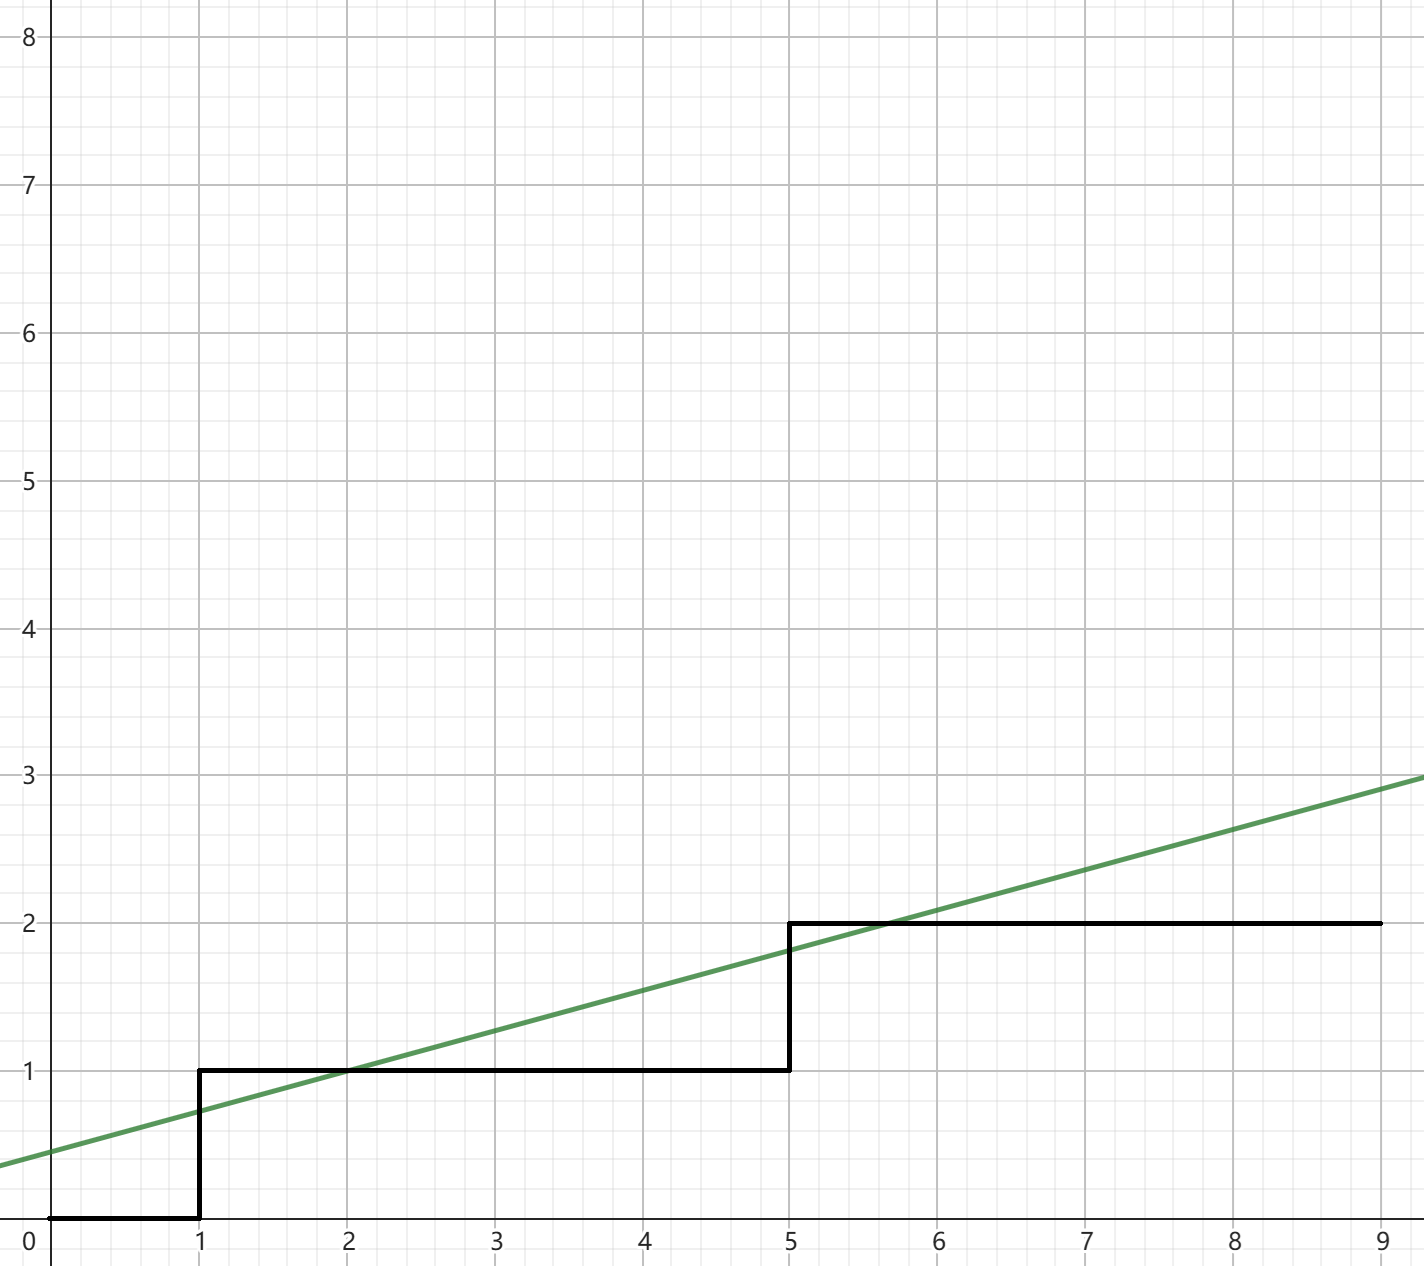
\includegraphics[scale=0.8]{1.png}

原理：考虑紧贴着斜线的折线的答案。每个 \verb|nd| 表示的是一段折线，你需要实现 \verb|operator+| 来计算出拼接两个折线之后的答案。注意，需要实现默认构造。

你需要传入的 \verb|dx| 和 \verb|dy| 表示向上和向右的折线的答案（也就是边界）。图中对应的折线为 $\texttt{RURRRRURRRR}$。

以对 $x$ 求和为例，通常的处理手段是在 \verb|dx| 时计算 $x=1$ 的答案，在 \verb|dy| 时更新辅助数组。

注意，如果 $x=0$ 处有答案，你需要手动计算它，并保证传入的 $b<m$。

如果这段向上的竖线对后面有影响，你可以在一开始先加一个 \verb|ksm(dy,...)|，但你仍然可能需要手动计算 $x=0$。

如果答案要取模，特别注意 $y$ 有可能比模数大！不卡时间请使用 \verb|int128|。

\lstinputlisting{code/数学/万能欧几里得_min of mod of linear.cpp}


\subsection{高斯整数类}

圆上整点的基础。

\lstinputlisting{code/数学/高斯整数类.cpp}

\subsection{Miller Rabin/Pollard Rho}

1s：$200$ 组 $10^{18}$。

如果你只需要做 \verb|int| 以内的分解，你可以改为

\lstinputlisting{code/数学/Miller Rabin_Pollard Rho.cpp}

\lstinputlisting{code/数学/Miller Rabin_Pollard Rho_2.cpp}


\newpage

\section{字符串}

\subsection{字典树（trie 树）}

\lstinputlisting{code/字符串/字典树(trie 树).cpp}

\subsection{AC 自动机}

注意 AC 自动机与 trie 不同的地方在于，根必须是 0。

题意：给你一个文本串 $S$ 和 $n$ 个模式串 $T_{1 \sim n}$，请你分别求出每个模式串 $T_i$ 在 $S$ 中出现的次数。

\lstinputlisting{code/字符串/AC 自动机.cpp}

\subsection{hash}

在调试时，可以把 \verb|base| 设置为 $10$ 的幂方便输出。可能建议把第一个模数也设置为 $1$，但未测试是否有奇怪的问题。但要注意，此时不应当使用接近 $10$ 的幂次的模数。

$O(n)$，$O(n)$。

建议抄 \verb|int128| 版本。目前来看，\verb|int128| 版本的既好写又快。

\verb|__int128| 版本：

\lstinputlisting{code/字符串/hash.cpp}

双模数版本：

特别注意这里 \verb|m| 数组预处理的不是幂次，而是幂次的相反数。

其返回值是两个 $32$ 位数拼接而成的，要改动比较麻烦。

\lstinputlisting{code/字符串/hash_2.cpp}


\subsection{KMP}

$O(n)$，$O(n)$。

\lstinputlisting{code/字符串/KMP.cpp}

\subsection{manacher}

$O(n)$，$O(n)$。

\verb|ex[i]| 表示以 $i/2$ 为回文中心的回文串长度。

如果 $t$ 可能包含 $\texttt{\$\#}$，你需要修改字符。

\lstinputlisting{code/字符串/manacher.cpp}

\subsection{SA}

$O((n+\sum)\log n)$，$O(n+\sum)$。

功能：查询两个后缀的 lcp。单次询问复杂度 $O(1)$。

下标从 $0$ 开始。

\lstinputlisting{code/字符串/SA.cpp}

\subsection{SAM}

$O(n\sum)$，$O(2n\sum )$。

\lstinputlisting{code/字符串/SAM.cpp}

\subsection{ukkonen 后缀树}

$O(n)$，$O(2n\sum )$。

\lstinputlisting{code/字符串/ukkonen 后缀树.cpp}

\subsection{ukkonen 后缀树（重构）}

\lstinputlisting{code/字符串/ukkonen 后缀树(重构).cpp}



\subsection{Z 函数}

表示每个后缀和母串的 lcp。

\lstinputlisting{code/字符串/Z 函数.cpp}



\subsection{最小表示法}

找到一个串的循环同构串中字典序最小的那个，将这个串直接变过去。常见应用：环哈希（基环树哈希）。

如果只需要找到起点下标，在 \verb|rotate| 前返回 $\min\{i,j\}$ 即可。

$O(n)$，$O(1)$。

\lstinputlisting{code/字符串/最小表示法.cpp}
\subsection{带通配符的字符串匹配}

原理：匹配等价于 $\sum (f_i-g_i)^2=0$。带通配符等价于 $\sum f_ig_i(f_i-g_i)^2=0$，展开即可。

这里也是较为推荐的 NTT 版本，直接实现任意长度的多项式相乘，便于一般情况的运用。不需要提前做任何 init。

\lstinputlisting{code/字符串/带通配符的字符串匹配.cpp}

快一些的版本，手动拆开了多项式乘法。

\lstinputlisting{code/字符串/带通配符的字符串匹配_2.cpp}
\newpage

\section{图论}

\subsection{最小生成树相关}

\subsubsection{切比雪夫距离最小生成树}

原理：先转曼哈顿距离，再用曼哈顿的板子。

$O(n\log n)$，$O(n)$。

\lstinputlisting{code/图论/最小生成树相关/切比雪夫距离最小生成树.cpp}

\subsubsection{最小乘积生成树}

题意：每条边有两个属性 $x_i,y_i$，你需要最小化 $(\sum x_i)(\sum y_i)$。

你需要实现的是 \verb|sol1|，即按照 $val$ 为权值的答案。$val_i$ 是根据 $x_i,y_i$ 计算的。

\lstinputlisting{code/图论/最小生成树相关/最小乘积生成树.cpp}

\subsubsection{最小斯坦纳树}

题意：让给定点集连通的最小生成树（不要求全图连通）

$O(3^kn+2^km\log m)$。

分为有方案与无方案两个版本，点标号 $[0,n)$。

\lstinputlisting{code/图论/最小生成树相关/最小斯坦纳树.cpp}


\subsection{最短路相关}

\subsubsection{全源最短路与判负环}

使用 floyd 实现全源最短路与判负环。注意边权较大时可能需要考虑 \verb|int128|.

\lstinputlisting{code/图论/最短路相关/全源最短路与判负环.cpp}

\subsubsection{Dijkstra/SPFA/Johnson}

Johnson 不适用于图中存在负环的情况，因为负环不一定是可以经过的。

$O(nm\log m)$，$O(n+m)$。

\lstinputlisting{code/图论/最短路相关/Dijkstra_SPFA_Johnson.cpp}
\subsubsection{无向图最小环}

原理：floyd 外层循环本质是计算只经过 $\le k$ 的点的最短路。因此枚举环上标号最大的，在做这一轮转移之前正好是不经过它的最短路。

$O(n^3)$，$O(n^2)$。

\lstinputlisting{code/图论/最短路相关/无向图最小环.cpp}

\subsubsection{输出负环}

\lstinputlisting{code/图论/最短路相关/输出负环.cpp}


\subsection{二分图与网络流建图}

以下约定，若为二分图则 $n,m$ 表示两侧点数，否则仅 $n$ 表示全图点数。

\subsubsection{二分图边染色}

留坑待填。

结论：$\Delta(G)\le \chi'(G) \le \Delta(G)+1$，二分图时 $\chi'(G)=\Delta(G)$。$\Delta(G)$ 为图的最大度。

\subsubsection{二分图最小点集覆盖}

$ans=\text{maxmatch}$，方案如下。

\lstinputlisting{code/图论/二分图与网络流建图/二分图最小点集覆盖.cpp}

\subsubsection{二分图最大独立集}

$ans=n+m-\text{maxmatch}$，方案是最小点集覆盖的补集。

\subsubsection{二分图最小边覆盖}

$ans=n+m-\text{maxmatch}$，方案是最大匹配加随便一些边（用于覆盖失配点）。无解当且仅当有孤立点，算法会视为单选孤立点（无边）。这个定理对一般图也成立。

\subsubsection{有向无环图最小不相交链覆盖}

$ans=n-\text{maxmatch}$，其中二分图建图方法是拆入点和出点（实现时直接跑一次二分图就行，不用额外处理），注意\textbf{不}需要传递闭包。方案如下。

\lstinputlisting{code/图论/二分图与网络流建图/有向无环图最小不相交链覆盖.cpp}

\subsubsection{有向无环图最大互不可达集}

$ans=n-\text{maxmatch}$，其中二分图建图方法是拆入点和出点（实现时直接跑一次二分图就行，不用额外处理），注意\textbf{需要}传递闭包。方案？

\subsubsection{最大权闭合子图}

若 $v_i>0$，$s\to i$ 流量 $v_i$；若 $v_i<0$，$i\to t$ 流量 $-v_i$。若原图 $u\to v$ 可花费 $w$ 代价违抗，流量 $w$，否则 $+\infty$ 。答案为 $\sum\limits_{v_i>0} v_i-\text{maxflow}$。方案？

\subsection{匹配与网络流相关代码}

\subsubsection{二分图最大权匹配}

\lstinputlisting{code/图论/匹配与网络流相关代码/二分图最大权匹配.cpp}

\subsubsection{一般图最大匹配}

\lstinputlisting{code/图论/匹配与网络流相关代码/一般图最大匹配.cpp}

\subsubsection{一般图最大权匹配}

$n=400$：UOJ 600ms, Luogu 135ms

\lstinputlisting{code/图论/匹配与网络流相关代码/一般图最大权匹配.cpp}

\subsubsection{网络流}

输出方案部分几乎没有验证过。

包含多种费用流方案，spfa，dijkstra，以及 capacity scaling 的 spfa。

\lstinputlisting{code/图论/匹配与网络流相关代码/网络流.cpp}


\subsubsection{假带花树}

一种错误的一般图最大匹配算法，但较难卡掉。推荐在时间不足时作为乱搞使用。

\lstinputlisting{code/图论/匹配与网络流相关代码/假带花树.cpp}

\subsubsection{Stoer-Wagner 全局最小割}

无向图 $G$ 的最小割为：一个去掉后可以使 $G$ 变成两个连通分量，且边权和最小的边集的边权和。

$O(n^3)$。可优化到 $O(nm\log n)$。

\lstinputlisting{code/图论/匹配与网络流相关代码/Stoer-Wagner 全局最小割.cpp}

\subsubsection{最小割树}

结论：两个点之间的最小割等于最小割树上两点间最小边权。

直接返回任意两点最小割。

\lstinputlisting{code/图论/匹配与网络流相关代码/最小割树.cpp}

\subsection{缩点相关}

\subsubsection{双极分解}

无向图，图点双连通时对任意 $s,t$ 存在。

含义：确定一个拓扑序，使得按这个拓扑序定向后，入度为 $0$ 的只有 $s$，出度为 $0$ 的只有 $t$。

\lstinputlisting{code/图论/缩点相关/双极分解.cpp}

\subsubsection{点双}

一些结论：

判定一个图里是否有（点不重复）偶环：看其所有点双，若存在点数为偶数的或边数多于点数的点双，则存在偶环。

（无自环时）点双的边不交，边双的点不交。点双内的总点数 $O(n)$，总边数为 $m$，边双内的总点数为 $n$，总边数不超过 $m$。

关于板子本身：

所有标号从 $0$ 开始。

构造函数传入邻接表和边数，其中 \verb|pair| 的 \verb|second| 是边的标号，正反向编号相同，允许不连续但不能大于等于 $m$。

不能处理有自环的情况。你可以直接在图中删除自环后传入。可以处理有重边的情况。

\verb|bcc_node|：每个点双包含的点（已验证）；
\verb|bcc_edge|：每个点双包含的边；
\verb|bcc_n|：新图点数；
\verb|ct|：是否割点（已验证）；
\verb|blk|：边所属点双标号。

\lstinputlisting{code/图论/缩点相关/点双.cpp}

\subsubsection{边双}

所有标号从 $0$ 开始。

构造函数传入邻接表和边数，其中 \verb|pair| 的 \verb|second| 是边的标号，正反向编号相同，允许不连续但不能大于等于 $m$。

可以处理有重边和自环的情况。

\verb|bcc_node|：每个边双包含的点（已验证）；
\verb|bcc_edge|：每个边双包含的边；
\verb|bcc_n|：新图点数；
\verb|cur_e|：新图边表；
\verb|ct|：是否割边；
\verb|blk|：点所属边双标号。

\lstinputlisting{code/图论/缩点相关/边双.cpp}

\subsubsection{Tarjan 强连通分量}

未经验证。

所有标号从 $0$ 开始。

构造函数传入邻接表，其中 \verb|pair| 的 \verb|second| 是边的标号。

与点边双不同的是，你可以任意传入 \verb|second|，代码中不会使用它，仅用于新图区分边。

可以处理有重边和自环的情况。

\verb|cc_node|：每个 SCC 包含的点（已验证）；
\verb|cc_n|：新图点数；
\verb|cur_e|：新图边表；
\verb|blk|：点所属 SCC 标号。

\lstinputlisting{code/图论/缩点相关/Tarjan 强连通分量.cpp}

\subsubsection{动态强连通分量}

给出一个加边序列，\verb|solve| 会返回每个时间进入强连通分量的边。点标号范围是 $[0,n)$

\lstinputlisting{code/图论/缩点相关/动态强连通分量.cpp}

\subsubsection{圆方树}

题意：求仙人掌上两点最短路。

$O(n+m)$，$O(n+m)$。

\lstinputlisting{code/图论/缩点相关/圆方树.cpp}

\subsubsection{广义圆方树}

建议使用点双来做这个。你只需要对每个点双建一个虚点，向点双内所有原点连边，就得到了广义圆方树。

\lstinputlisting{code/图论/缩点相关/广义圆方树.cpp}

\subsubsection{$2$-sat}

支持添加一个条件 \verb|add(u, x, v, y)|，表示 $a_u=x\Rightarrow a_v=y$。支持设定一个变量的值。

$O(n+m)$，$O(n+m)$。

\lstinputlisting{code/图论/缩点相关/2-sat.cpp}


\subsubsection{Kosaraju 强连通分量（bitset 优化）}

实用意义不大。

$O(\frac{n^2}w)$，$O(\frac {n^2}w)$。

\lstinputlisting{code/图论/缩点相关/Kosaraju 强连通分量(bitset 优化).cpp}



\subsection{树上问题}

\subsubsection{换根 dp}

$[0,n)$。

zero 版：

\lstinputlisting{code/图论/树上问题/换根 dp.cpp}

合并版：

\lstinputlisting{code/图论/树上问题/换根 dp_2.cpp}


\subsubsection{轻重链剖分/DFS 序 LCA}

首先 \verb|init(n)|，然后正常存边（$[1,n]$），然后 \verb|fun(root)|。

\verb|get_path| 会返回这条路径上的 \verb|dfn| 区间。

\lstinputlisting{code/图论/树上问题/轻重链剖分_DFS 序 LCA.cpp}

\subsubsection{换根树剖}

本质是对普通树剖在换根后的子树进行分类讨论。

设预处理的根是 $u$，当前根是 $v$，那么 $w$ 的子树如下：

\begin{enumerate}
	\item $w=v$，\verb|dfn| 区间为 $[1,n]$。
	\item $w$ 在 $u,v$ 之间，\verb|dfn| 区间为 $[1,n]$ 去掉 $w$ 前往 $v$ 方向的子树。找到这个子树的方法见 \verb|find| 函数。
	\item 其余情况，\verb|dfn| 区间和原来一致。
\end{enumerate}

\lstinputlisting{code/图论/树上问题/换根树剖.cpp}
$O(n+q\log n)$，$O(n)$。


\subsubsection{毛毛虫剖分}
毛毛虫剖分，一种由轻重链剖分（HLD）推广而成的树上结点重标号方法，支持修改 / 查询一只毛毛虫的信息，并且可以对毛毛虫的身体和足分别修改 / 查询不同信息 .

严格强于树剖，而且复杂度和树剖一样哦！

一些定义（默认在一棵树上）：

毛毛虫：一条链和与这条链邻接的所有结点构成的集合 .
虫身（身体）：毛毛虫的链部分 .
虫足（足）：毛毛虫除虫身的部分 .
重标号方法
首先重剖求出重链 .
DFS，若现在处理到结点 u：
若 u 还未被标号，则为其标号 .
若 u 是重链头，遍历这条重链，将邻接这条链的结点依次标号 .
先递归重儿子，再递归轻儿子 .
重标号性质
对于重链，除链头外的结点标号连续 .
对于任意结点，其轻儿子标号连续 .
对于以重链头为根的子树，与这条重链邻接的所有结点标号连续 .
这样就可以随便维护毛毛虫信息了，顺便还能维护链信息，子树信息等 .

时间复杂度同轻重链剖分 .

以 SAM 为例，若我们只保留所有的转移边 $(u,v)$ ，满足到达 $u$ 的路径数目大于到达 $v$ 的路径数目一半，且从 $v$ 出发的路径数目大于从 $u$ 出发的路径数目一半，这样剩余的子图显然会形成若干条链，且每个点恰好在一条链上。这样，我们容易证明，从根结点出发的任何一条路径，至多经过 $O(\log n)$ 条不在链上的转移边（也意味着至多经过 $O(\log n)$ 条链） 。

以下是一段示例代码，展示了将一条链对应区间取出来的过程

\lstinputlisting{code/图论/树上问题/毛毛虫剖分.cpp}


\subsubsection{树上启发式合并，DSU on tree}

一种过时的、基于两次 \verb|dfs| 的写法，在复杂度要求不严时不如直接存储 \verb|set|。

流程：

\begin{enumerate}
	\item \verb|dfs| 轻子树计算答案，并清空全局统计信息。
	\item \verb|dfs| 重子树统计答案和全局信息。
	\item \verb|dfs| 轻子树统计全局信息。
\end{enumerate}

\lstinputlisting{code/图论/树上问题/树上启发式合并，DSU on tree.cpp}

\subsubsection{长链剖分（$k$ 级祖先）}

$O(n\log n+q)$，$O(n)$。

\lstinputlisting{code/图论/树上问题/长链剖分(k 级祖先).cpp}

\subsubsection{长链剖分（dp 合并）}

一种常见的实现方法是用指针指向同一片数组区域，使得从链头到链尾正好指向连续的一段数组，就不需要计算偏移量了。

$O(n)$，$O(n)$。

\lstinputlisting{code/图论/树上问题/长链剖分(dp 合并).cpp}
\subsubsection{LCT}

$O(n\log n)$，$O(n)$。

\verb|makeroot| 会变根，\verb|split| 会把 $y$ 变根，\verb|findroot| 会把根变根，\verb|link| 会把 $x,y$ 变根（$y$ 是新的），\verb|cut| 会把 $x,y$ 变根（$x$ 是新的），注意 \verb|swap| 子节点可能要 \verb|pushup|。

代码为动态割边割点。

\lstinputlisting{code/图论/树上问题/LCT.cpp}


\subsubsection{带子树的 LCT}

$O(n\log n)$，$O(n)$。

你需要实现的是 \verb|info| 类的 \verb|+,+=,-=|。

\begin{enumerate}
	\item \verb|info| 维护的是从上往下的一条链以及这条链挂着的所有轻子树的信息。
	\item \verb|a+b| 表示两条链合并后的信息，其中 $a$ 接近根。
	\item \verb|a+=b| 表示一条链合并了一个轻子树，即 $b$ 是 $a$ 链尾的子结点。
	\item \verb|a-=b| 表示一条链移除了一个轻子树，即 $b$ 是 $a$ 链尾的子节点。
\end{enumerate}

如果有边权，将边 $(u,v)$ 当成点并与 $u,v$ 分别连边。

代码对应题意：

对于满足 $0 \leq e \leq N - 2$ 的整数 $e$，定义 $f_e(x) = b_e x + c_e$。

设 $e_0, e_1, \ldots, e_k$ 为从顶点 $x$ 到顶点 $y$ 的简单路径上的边，按顺序排列，并定义
\[
	P(x, y) = f_{e_0}(f_{e_1}(\ldots f_{e_k}(a_y) \ldots)).
\]

按给定顺序处理 $Q$ 个查询。查询有两种类型：

\begin{itemize}
	\item $\texttt{0 w x r}$：将 $a_w$ 更新为 $x$，然后输出
	      \[
		      \left( \sum_{v=0}^{N-1} P(r, v) \right) \mod 998244353.
	      \]
	\item $\texttt{1 e y z r}$：将 $(b_e, c_e)$ 更新为 $(y, z)$，然后输出
	      \[
		      \left( \sum_{v=0}^{N-1} P(r, v) \right) \mod 998244353.
	      \]
\end{itemize}

\lstinputlisting{code/图论/树上问题/带子树的 LCT.cpp}

\subsubsection{动态 dp（全局平衡二叉树）}

意义不大。

$O((n+q)\log n)$，$O(n)$。

\lstinputlisting{code/图论/树上问题/动态 dp(全局平衡二叉树).cpp}

\subsubsection{全局平衡二叉树（修改版）}

$O((n+q)\log n)$，$O(n)$。

\lstinputlisting{code/图论/树上问题/全局平衡二叉树(修改版).cpp}

\subsubsection{虚树}

传入点标号列表，返回虚树边表。自动认为 $1$ 是根，标号从 $1$ 开始。

需要注意的是：在清空的时候需要同时考虑点列表和边表，都清空一下。

你需要提供的是：\verb|dep|,\verb|lca|,\verb|dfn|。

$O(n+\sum k\log n)$，$O(n)$。

\lstinputlisting{code/图论/树上问题/虚树.cpp}

\subsubsection{点分治}

点分治板子的参考意义不大。

$O(n\log n)$，$O(n)$。

\lstinputlisting{code/图论/树上问题/点分治.cpp}

\subsubsection{点分树}

核心结论：点分树上 lca 出现在原树路径上。

$O(n\log^2 n)$，$O(n\log n)$。

\lstinputlisting{code/图论/树上问题/点分树.cpp}

圆环修改和单点查询：

\lstinputlisting{code/图论/树上问题/点分树_2.cpp}

单点修改和圆环查询：

\lstinputlisting{code/图论/树上问题/点分树_3.cpp}

\subsubsection{（基环）树哈希}

有根树返回每个子树的哈希值，无根树返回树的哈希值（长度至多为 $2$ 的 \verb|vector|），基环树返回图的哈希值（长度等于环长的 \verb|vector|）。

\lstinputlisting{code/图论/树上问题/(基环)树哈希.cpp}

\subsection{欧拉路相关}

\subsubsection{构造：字典序最小}

\lstinputlisting{code/图论/欧拉路相关/构造：字典序最小.cpp}

\subsubsection{回路/通路构造}

$O(n+m)$，$O(n+m)$。

\lstinputlisting{code/图论/欧拉路相关/回路_通路构造.cpp}

\subsubsection{回路计数（BEST 定理）/生成树计数}

$O(n^3)$，$O(n^2)$。

以 $u$ 为起点的欧拉回路个数 $sum=T(u)\times \prod\limits_{v=1}^n(out(v)-1)!$，其中 $T(u)$ 是以 $u$ 为根的内向树个数（出度矩阵-邻接矩阵），$out(v)$ 是 $v$ 的出度。若允许循环同构（如 $1\to 2\to 1\to 3\to 1$ 与 $1\to 3\to 1\to 2\to 1$），还需多乘 $out(u)$。

这里的部分代码是未经验证的。

\lstinputlisting{code/图论/欧拉路相关/回路计数(BEST 定理)_生成树计数.cpp}

\subsection{三/四元环计数}

不能处理有重边和自环的情况。

$O(m\sqrt m)$，$O(n+m)$。

注意四元环数的是边四元环。点四元环需要去掉四点完全图个数*2，似乎不太能做？

三元环是可以枚举的，你可以在 \verb|ans| 改变时记录三元环 $(i,u,v)$。

\lstinputlisting{code/图论/三_四元环计数.cpp}

\subsection{支配树}

$u$ 支配 $v$ 指的是从 $S$ 到 $v$ 的路径必然经过 $u$。支配树是保持支配关系不变的树，其中 $s$ 是根，$idom[u]$ 是 $u$ 的父节点。

DAG 版：$O(m\log n)$，$O(n\log n)$。

\lstinputlisting{code/图论/支配树.cpp}

一般图：标号从 $1$ 开始。

\lstinputlisting{code/图论/支配树_2.cpp}

\subsection{prufer 与树的互相转化}

$O(n)$，$O(n)$。

\lstinputlisting{code/图论/prufer 与树的互相转化.cpp}


\subsection{最小密度环}

求所有环中边权和除以边数最少的，$O(nm)$。更常用的做法是二分 spfa。

\lstinputlisting{code/图论/最小密度环.cpp}


\subsection{点染色}

结论：$\chi(G)\le \Delta(G)+1$，其中 $\Delta(G)$ 是图的最大度。只有奇圈和完全图取等。

构造方案只能爆搜。

\lstinputlisting{code/图论/点染色.cpp}

\subsection{最大独立集}

爆搜。

\lstinputlisting{code/图论/最大独立集.cpp}

\subsection{弦图}

单纯点：$v$ 和 $v$ 邻点构成团。

完美消除序列：$v_i$ 在 $\{v_i,v_{i+1},\cdots,v_n\}$ 为单纯点。

$N(v_i)=\{v_j|j>i\land (v_i,v_j)\in E\}$，$next(v_i)$ 为 $N(v_i)$ 最靠前的点。

极大团一定是 $\{v\}\cup N(v)$ 。

最大团大小等于色数。

弦图判定：等价于是否存在完美消除序列。首先求出一个完美消除序列，然后判定是否合法。

判定方法：设 $v_{i+1},\cdots,v_n$ 中与 $v_i$ 相邻的依次为 $v'_1,\cdots,v'_m$。只需判断是否 $v_1'$ 与 $v'_2,\cdots,v'_m$ 相邻。

LexBFS 算法（我不会写）

每个点有一个字符串 label，初始为 $0$。从 $i=n$ 到 $i=1$ 确定，选 label 字典序最大的 $u$，再把 $u$ 邻点的 label 后面接一个 $i$。

最大势算法：从 $v_n$ 求到 $v_1$，设 $label_i$ 表示 $i$ 与多少个已选点相邻，每次选 $label_i$ 最大的点。

弦图极大团：$\{v|\forall next(w)=v,|N(v)|\ge |N(w)|\}$。选出的集合为基本点，按上述极大团构造。

弦图染色：从 $v_n$ 到 $v_1$ 依次选最小可染的色。

最大独立集：从 $v_1$ 到 $v_n$ 能选就选。

最小团覆盖：设最大独立集为 $\{p_m\}$，最小团覆盖为 $\{\{p_i\}\cup N(p_i)\}$。

区间图：两个区间有边当且仅当交集非空。

区间图是弦图。

代码如下：

\lstinputlisting{code/图论/弦图.cpp}




\newpage

\section{计算几何}

\subsection{自适应 simpson 法}

\verb|sim(l,r)| 计算 $\int_l^r f(x)\dif x$

\lstinputlisting{code/计算几何/自适应 simpson 法.cpp}

\subsection{计算几何全}

功能其实比较少，因为实际遇到的几何题不多。最有用的可能是闵可夫斯基和合并凸包，和常规的线段判交之类的。其余功能最好直接使用 HDU 板。

\lstinputlisting{code/计算几何/计算几何全.cpp}

另附一份支持二分斜率的代码。这里维护的是 $(x,y)$，其中 $y=C+x^2$，因此 $x$ 整体增加会影响 $y$。
\lstinputlisting{code/计算几何/计算几何全_2.cpp}
\newpage

\section{杂项}

\subsection{枚举大小为 $k$ 的集合}

思路：通过进位创造 $1$，再把一串 $1$ 移到最后。

\lstinputlisting{code/杂项/枚举大小为 k 的集合.cpp}
\subsection{min plus 卷积}

计算 $c_i=\min\limits_{j=0}^i a_j+b_{i-j}$。

要求 $b$ 是凸的，即 $b_{i+1}-b_i$ 不降。

\lstinputlisting{code/杂项/min plus 卷积.cpp}

\subsection{所有区间 GCD}

需要自定义 \verb|fun|，如 $\gcd$，$\operatorname{and}$，$\operatorname{or}$。

\lstinputlisting{code/杂项/所有区间 GCD.cpp}
\subsection{整体二分（区间 $k$-th）}

$O((n+q)\log a)$，$O(n+q)$。

\lstinputlisting{code/杂项/整体二分(区间 k-th).cpp}

\subsection{高精度}

除法和取模有点问题，但 gcd 是对的。

\lstinputlisting{code/杂项/高精度.cpp}

\subsection{分散层叠算法（Fractional Cascading）}

$O(n+q(k+\log n))$，$O(n)$。

给出 $k$ 个长度为 $n$ 的有序数组。

现在有 $q$ 个查询：给出数 $x$，分别求出每个数组中大于等于 $x$ 的最小的数（非严格后继）。

若后继不存在，则定义为 $0$。你需要在线地回答这些询问。

\lstinputlisting{code/杂项/分散层叠算法(Fractional Cascading).cpp}

\subsection{圆上整点（二平方和定理）}

$x^2+y^2=n$ 的整数解的数目的四分之一 $f(n)$ 是积性数论函数，且对于{\bf{素数幂}}有：
$f(p^k)=\begin{cases}
		1            & p=2               \\
		k+1          & p\equiv 1 \pmod 4 \\
		(k+1)\bmod 2 & p\equiv 3 \pmod 4
	\end{cases}$

以下代码给出所有的非负整数解。注意非负整数解个数不等于 $f(n)$。

时间复杂度为 $O(n^{\frac{1}{4}}+f(n))$，其中 $O(n^{\frac{1}{4}})$ 是 pollard-rho 的复杂度。

$f(n)$ 的量级不好分析，但不会超过约数个数 $O(d(n))\approx O(n^{\frac{1}{3}})$，且可以推测不能达到。实践上 $10^{18}$ 以内 $f(n)\le 3072$。

\lstinputlisting{code/杂项/圆上整点(二平方和定理).cpp}

\subsection{Stern-Brocot Tree}

你需要时刻保持传入的 $\dfrac{num}{den}$ 满足 $\gcd(num,den)=1$。

\lstinputlisting{code/杂项/Stern-Brocot Tree.cpp}

\subsection{快速取模}

\lstinputlisting{code/杂项/快速取模.cpp}

\subsection{IO 优化}

\lstinputlisting{code/杂项/IO 优化.cpp}
\subsection{手动开栈}

一种写法是文件开头放，但部分 OJ 会失效。

\lstinputlisting{code/杂项/手动开栈.cpp}

另一种写法是在 \verb|main| 开头写，但必须以 \verb|exit(0)| 结束程序。

以下两个应该有一个是对的，不对会 CE。

\lstinputlisting{code/杂项/手动开栈_2.cpp}

\subsection{德扑}

\verb|solve| 返回按照出现次数排序的 \verb|vector<int>|（$0$ 下标处为牌型），这样就可以字典序比较了。

\lstinputlisting{code/杂项/德扑.cpp}

\subsection{随机函数}

\verb|u64| $\to$ \verb|u64|

\lstinputlisting{code/杂项/随机函数.cpp}


\subsection{约数个数表}
\begin{table}[H]
	\centering
	\hspace*{-0.5cm}
	\begin{tabular}{|c|c|c|c|c|c|}
		\toprule
		$n$       & $n$ 前第一个质数 & $n$ 后第一个质数 & $\max\{\omega(n)\}$ & $\max\{d(n)\}$                    & $\pi(n)$           \\
		\midrule
		$10^{1}$  & $n-3$      & $n+1$      & $2$                 & $d(6) = 4$                        & $4$                \\\midrule
		$10^{2}$  & $n-3$      & $n+1$      & $3$                 & $d(60) = 12$                      & $25$               \\\midrule
		$10^{3}$  & $n-3$      & $n+13$     & $4$                 & $d(840) = 32$                     & $168$              \\\midrule
		$10^{4}$  & $n-27$     & $n+7$      & $5$                 & $d(7560) = 64$                    & $1229$             \\\midrule
		$10^{5}$  & $n-9$      & $n+3$      & $6$                 & $d(83160) = 128$                  & $9592$             \\\midrule
		$10^{6}$  & $n-17$     & $n+3$      & $7$                 & $d(720720) = 240$                 & $7.9\cdot 10^4$    \\\midrule
		$10^{7}$  & $n-9$      & $n+19$     & $8$                 & $d(8648640) = 448$                & $6.7\cdot 10^5$    \\\midrule
		$10^{8}$  & $n-11$     & $n+7$      & $8$                 & $d(73513440) = 768$               & $5.8\cdot 10^6$    \\\midrule
		$10^{9}$  & $n-63$     & $n+7$      & $9$                 & $d(735134400) = 1344$             & $5.1\cdot 10^7$    \\\midrule
		$10^{10}$ & $n-33$     & $n+19$     & $10$                & $d(6983776800) = 2304$            & $4.6\cdot 10^8$    \\\midrule
		$10^{11}$ & $n-23$     & $n+3$      & $10$                & $d(97772875200) = 4032$           & $4.2\cdot 10^8$    \\\midrule
		$10^{12}$ & $n-11$     & $n+39$     & $11$                & $d(963761198400) = 6720$          & $3.8\cdot 10^9$    \\\midrule
		$10^{13}$ & $n-29$     & $n+37$     & $12$                & $d(9316358251200) = 10752$        & $3.5\cdot 10^{10}$ \\\midrule
		$10^{14}$ & $n-27$     & $n+31$     & $12$                & $d(97821761637600) = 17280$       & $3.3\cdot 10^{11}$ \\\midrule
		$10^{15}$ & $n-11$     & $n+37$     & $13$                & $d(866421317361600) = 26880$      & $3\cdot 10^{12}$   \\\midrule
		$10^{16}$ & $n-63$     & $n+61$     & $13$                & $d(8086598962041600) = 41472$     & $2.8\cdot 10^{13}$ \\\midrule
		$10^{17}$ & $n-3$      & $n+3$      & $14$                & $d(74801040398884800) = 64512$    &                    \\\midrule
		$10^{18}$ & $n-11$     & $n+3$      & $15$                & $d(897612484786617600) = 103680$  &                    \\\midrule
		$10^{19}$ & $n-39$     & $n+51$     & $16$                & $d(9200527969062830400) = 161280$ &                    \\
		\bottomrule
	\end{tabular}
\end{table}
\subsection{NTT 质数}
\begin{table}[H]
	\centering
	\begin{tabular}{|c|c|c|c|c|}

		\toprule
		$p=r\times 2^k+1$     & $r$   & $k$  & $g$（最小原根） & 位数   \\
		\midrule
		$17$                  & $1$   & $4$  & $3$       & $2$  \\
		$97$                  & $3$   & $5$  & $5$       & $2$  \\
		$193$                 & $3$   & $6$  & $5$       & $3$  \\
		$257$                 & $1$   & $8$  & $3$       & $3$  \\
		$7681$                & $15$  & $9$  & $17$      & $4$  \\
		$12289$               & $3$   & $12$ & $11$      & $5$  \\
		$40961$               & $5$   & $13$ & $3$       & $5$  \\
		$65537$               & $1$   & $16$ & $3$       & $5$  \\
		$786433$              & $3$   & $18$ & $10$      & $6$  \\
		$5767169$             & $11$  & $19$ & $3$       & $7$  \\
		$7340033$             & $7$   & $20$ & $3$       & $7$  \\
		$23068673$            & $11$  & $21$ & $3$       & $8$  \\
		$104857601$           & $25$  & $22$ & $3$       & $9$  \\
		$167772161$           & $5$   & $25$ & $3$       & $9$  \\
		$469762049$           & $7$   & $26$ & $3$       & $9$  \\
		$998244353$           & $119$ & $23$ & $3$       & $10$ \\
		$1004535809$          & $479$ & $21$ & $3$       & $10$ \\
		$2013265921$          & $15$  & $27$ & $31$      & $10$ \\
		$2281701377$          & $17$  & $27$ & $3$       & $10$ \\
		$3221225473$          & $3$   & $30$ & $5$       & $10$ \\
		$75161927681$         & $35$  & $31$ & $3$       & $11$ \\
		$77309411329$         & $9$   & $33$ & $7$       & $11$ \\
		$206158430209$        & $3$   & $36$ & $22$      & $12$ \\
		$2061584302081$       & $15$  & $37$ & $7$       & $13$ \\
		$2748779069441$       & $5$   & $39$ & $3$       & $13$ \\
		$6597069766657$       & $3$   & $41$ & $5$       & $13$ \\
		$39582418599937$      & $9$   & $42$ & $5$       & $14$ \\
		$79164837199873$      & $9$   & $43$ & $5$       & $14$ \\
		$263882790666241$     & $15$  & $44$ & $7$       & $15$ \\
		$1231453023109121$    & $35$  & $45$ & $3$       & $16$ \\
		$1337006139375617$    & $19$  & $46$ & $3$       & $16$ \\
		$3799912185593857$    & $27$  & $47$ & $5$       & $16$ \\
		$4222124650659841$    & $15$  & $48$ & $19$      & $16$ \\
		$7881299347898369$    & $7$   & $50$ & $6$       & $16$ \\
		$31525197391593473$   & $7$   & $52$ & $3$       & $17$ \\
		$180143985094819841$  & $5$   & $55$ & $6$       & $18$ \\
		$1945555039024054273$ & $27$  & $56$ & $5$       & $19$ \\
		$4179340454199820289$ & $29$  & $57$ & $3$       & $19$ \\
		\bottomrule
	\end{tabular}

\end{table}
\subsection{公式}

向上取整的整除分块 $[i,\lfloor\dfrac{n-1}{\lceil\dfrac ni \rceil-1}\rfloor]$

$n$ 个点 $k$ 个连通块的生成树方案 $n^{k-2}\prod\limits_{i=1}^k siz_i$

$(x,y)$ 曼哈顿距离 $\to$ $(x+y,x-y)$ 切比雪夫距离

$(x,y)$ 切比雪夫距离 $\to$ $(\dfrac{x+y}{2},\dfrac{x-y}{2})$ 曼哈顿距离

$k\text{-th}\max\{S\}=\sum\limits_{T\subseteq S}(-1)^{|T|-k}\tbinom{|T|-1}{k-1}\min\{T\}$

Kummer's Theorem: $\tbinom{n+m}{n}$ 含 $p~(p\in \text {prime})$ 的次数是 $n+m$ 在 $p$ 进制下的进位数

$\ln (1-x^V)=-\sum\limits_{i\ge1}\dfrac{x^{Vi}}{i}$

$x^{\bar n}=\sum\limits_i S_1(n,i)x^i$

$\begin{cases}x\equiv a_1\pmod {m_1}\\x\equiv a_2\pmod {m_2}\\\cdots\\x\equiv a_n\pmod {m_n}\end{cases}$

$V-E+F=2$，$S=n+\frac s2-1$。（$n$ 为内部，$s$ 为边上）

用途：对于相邻的不相等的值，在中间画一条线（最外也画），$\text{连通块个数}=1+E-V+\text{内部框个数}$

注意全都是不含矩形边界上的。

卡特兰三角：由 $n$ 个 $-1$ 和 $m$ 个 $1$ 组成一个序列，满足所有前缀和小于 $k$ 的方案数（$k\le m\le n+k-1$）：$\binom{n+m}{m}-\binom{n+m}{m-k}$

贝尔数（划分集合方案数）EGF：$\exp(e^x-1)$，$B_n=\sum\limits_{i=0}^n S_2(n,i)$，伯努利数 EGF：$\dfrac{x}{e^x-1}$

$S_1(i,m)$ EGF：$\dfrac{(\sum\limits_{i\ge 0}\dfrac{x^i}i)^m}{m!}$，$S_2(i,m)$ EGF：$\dfrac{(e^x-1)^m}{m!}$。$S_2(n,m)=[x^n]x^m(\prod\limits_{i=1}^m(1-ix))^{-1}$，$S_2(n,m)\equiv [n-m\&\lfloor\frac{m-1}{2}\rfloor=0]\pmod 2$。

多项式牛顿迭代：如果已知 $G(F(x))\equiv0\pmod{x^{2n}}$，$G(F_*(x))\equiv0\pmod {x^n}$，则有 $F(x)\equiv F_*(x)-\frac{G(F_*(x))}{G'(F_*(x))}\pmod{x^{2n}}$。求导时孤立的多项式视为常数。

$\int_0^1 t^a(1-t)^b\mathrm{d}t=\dfrac{a!b!}{(a+b+1)!}$，$\sum\limits_{i=0}^{n-1}i^{\underline{k}}=\dfrac{n^{\underline{k+1}}}{k+1}$

Burnside 引理：等价类数量为 $\sum\limits_{g\in G}\dfrac{X^g}{|G|}$，$X^g$ 表示 $g$ 变换下不动点的数量。

Polya 定理：染色方案数为 $\sum\limits_{g\in G}\dfrac{m^{c(g)}}{|G|}$，其中 $c(g)$ 表示 $g$ 变换下环的数量。

假设已经只保留了一个牛人酋长，其名字为 $A=a_1a_2\cdots a_l$。

假设王国旁边开了一座赌场，每单位时间（就称为“秒”吧）会有一个赌徒带着 $1$ 铜币进入赌场。

赌场规则很简单：支付 $x$ 铜币赌下一秒会唱出 $y$，如果猜对了就返还 $nx$ 铜币，否则钱就没了。

每个赌徒会如下行动：支付 $1$ 铜币赌下一秒会唱出 $a_1$，如果赌对了就支付得到的 $n$ 铜币赌下一秒会唱出 $a_2$，如果还对了就支付得到的 $n^2$ 铜币赌下一秒会唱出 $a_3$，等等，以此类推，最后支付 $n^{l-1}$ 铜币赌下一秒会唱出 $a_l$。

一旦连续唱出了 $a_1a_2\cdots a_l$，赌场老板就会认为自己亏大了而关门，并驱散所有赌徒。

那么关门前发生了什么呢？以 $A=\{1,4,1,5,1,1,4,1\},n=5$ 为例：

- 最后一位赌徒拿着 $5$ 铜币离开；
- 倒数第三位赌徒拿着 $5^3$ 铜币离开；
- 倒数第八位赌徒拿着 $5^8$ 铜币离开；
- 其他所有赌徒空手而归。

我们可以发现 $1,3$ 恰好是原序列的所有 border 的长度，而且对于其他的名字也有这样的规律。

这时候最神奇的一步来了：由于这个赌博游戏是公平的，因此赌场应该期望下不赚不赔，因此关门时期望来了 $5+5^3+5^8$ 个赌徒，因此期望需要 $5+5^3+5^8$ 单位时间唱出这个名字。

同理，即可知道对于一般的 $A$，答案为：

$$\sum\limits_{a_1a_2\cdots a_c=a_{l-c+1}a_{l-c+2}\cdots a_l} n^c$$


\newpage

\section{语言基础}

\subsection{Makefile}

\lstinputlisting{code/语言基础/Makefile.cpp}
\subsection{debug.h}

\lstinputlisting{code/语言基础/debug.h.cpp}

\subsection{初始代码}

\lstinputlisting{code/语言基础/初始代码.cpp}

抄写完 \verb|debug.h| 后，补充于 \verb|using namespace std;| 下一行：

\lstinputlisting{code/语言基础/初始代码_2.cpp}


\subsection{bitset}

\lstinputlisting{code/语言基础/bitset.cpp}

输出：

\begin{verbatim}
0011000000
1010010000
1010010000
0000100101
\end{verbatim}

\subsection{pb\_ds 和一些奇怪的用法}

\lstinputlisting{code/语言基础/pb__ds 和一些奇怪的用法.cpp}

\subsection{python 使用方法}

注意事项：python 容易爆栈，且引用与赋值较为混乱。注意局部变量的 \verb|global| 怎么写（如果需要修改全局内容）。

文件操作

\lstinputlisting[language=python]{code/语言基础/python 使用方法.py}


类的构造，重载运算符
\lstinputlisting[language=python]{code/语言基础/python 使用方法_2.py}

初始代码

\lstinputlisting[language=python]{code/语言基础/python 使用方法_3.py}

\newpage

\section{其他人的板子（补充）}
\subsection{最小树形图}

\lstinputlisting{code/其他人的板子(补充)/最小树形图.cpp}
\subsection{MTT+exp}

\lstinputlisting{code/其他人的板子(补充)/MTT+exp.cpp}

\subsection{半平面交}

\lstinputlisting{code/其他人的板子(补充)/半平面交.cpp}

\subsection{多项式复合 (yurzhang)}

$O(n\log n\sqrt{n\log n})$，奇慢无比，慎用

\lstinputlisting{code/其他人的板子(补充)/多项式复合 (yurzhang).cpp}

\subsection{下降幂多项式乘法}

$O(n\log n)$。

\lstinputlisting{code/其他人的板子(补充)/下降幂多项式乘法.cpp}

\subsection{弦图找错}

\lstinputlisting{code/其他人的板子(补充)/弦图找错.cpp}

\subsection{最长公共子序列}

复杂度 $O(\frac{nm}{\omega})$。

\lstinputlisting{code/其他人的板子(补充)/最长公共子序列.cpp}

另一个实现

\lstinputlisting{code/其他人的板子(补充)/最长公共子序列_2.cpp}

\subsection{区间 LIS（排列）}

在线：


\lstinputlisting{code/其他人的板子(补充)/区间 LIS(排列).cpp}


离线：

\lstinputlisting{code/其他人的板子(补充)/区间 LIS(排列)_2.cpp}

\subsection{区间 LCS}

$s_{[0,a)}$ 和 $t_{[b,c)}$ 的 LCS

\lstinputlisting{code/其他人的板子(补充)/区间 LCS.cpp}
\end{document}
